\documentclass[9pt, conference, a4paper, compsocconf]{IEEEtran}
\usepackage{amsmath,amsxtra,amssymb,amsthm,latexsym,amscd,amsfonts}
\usepackage[utf8]{vietnam}
\usepackage[top=2.7cm, bottom = 5.4cm, left=2.72cm, right = 2.85cm]{geometry}
\headsep = 0.7cm
\headheight = 1.0cm 
\footskip = 1.0cm
\voffset = -0.74 cm 
%%%%
\usepackage{balance}

\usepackage{fancyhdr}
\pagestyle{fancy}
\usepackage{cite}
\usepackage{algorithmic}
\usepackage{graphicx}
\usepackage{textcomp}
\usepackage{booktabs}   
\usepackage{tabularx}  
\usepackage{xcolor}
\usepackage{amsmath,amsxtra,amssymb,amsthm,latexsym,amscd,amsfonts}
\usepackage{pgfplots}
\usepackage{multirow}
\usepackage{subcaption}
\pgfplotsset{compat=1.17} 

\usepackage{tikz}
\usetikzlibrary{positioning}  
\usetikzlibrary{arrows.meta}  
\usetikzlibrary{shapes}      
\usetikzlibrary{calc}      
\usetikzlibrary{fit}          
\usepackage[english]{babel} %Figure ... English (có thể bỏ đi nếu bài viết tiếng Việt)
\usepackage{fancyhdr}
\pagestyle{fancy}
%\renewcommand{\chaptermark}[1]{\markboth{\MakeUppercase{#1}}{}}
\renewcommand{\sectionmark}[1]{\markright{\MakeUppercase{#1}}{}}
\renewcommand{\headrulewidth}{0pt}
\ifCLASSINFOpdf
\usepackage[pdftex]{graphicx}
  \DeclareGraphicsExtensions{.pdf,.jpeg,.png,.jpg}
\else
\usepackage[dvips]{graphicx}
  \DeclareGraphicsExtensions{.eps}
\fi
\usepackage{array}

\usepackage{caption}
\captionsetup{
  font={footnotesize}, 
  labelfont=bf,
  justification=centering,
  singlelinecheck=false
}
\usepackage[font=footnotesize]{subfig}

\makeatletter
\def\ps@IEEEtitlepagestyle{%
\def\@oddhead{\hfil \small{\textit{Hội thảo khoa học Quốc gia về Trí tuệ nhân tạo 2026 (FJCAI) - Cần Thơ, 27-28/3/2026}\hfil}%
	\def\@evenhead{\hfil\small{\textit{Hội thảo khoa học quốc gia về Trí tuệ nhân tạo 2026 (FJCAI) - Cần Thơ, 27-28/3/2026}\hfil}}%
		\def\@oddfoot{\scriptsize \thepage \hfil }%
		\def\@evenfoot{\scriptsize \hfil \thepage}
	}
}

\def\@maketitle{%
  \newpage
  \null
  \begin{center}%
    {%
      \fontsize{16}{18}\selectfont
      \bfseries \@title \par
    }%
    \vskip 4em%
    {%
    \fontsize{9}{3.5}\selectfont
      
      \begin{tabular}[t]{c}%
        \@author
      \end{tabular}\par
    }%
  \end{center}%
  \par
}

\renewenvironment{abstract}
  {\normalfont
   \if@twocolumn
     \@IEEEabskeysecsize\bfseries\textit{\abstractname}: 
   \else
     \begin{center}\@IEEEabskeysecsize\textbf{\abstractname}\end{center}
     \@IEEEabskeysecsize
     \setlength{\parindent}{0pt}   % ← tắt thụt đầu dòng
     \noindent
   \fi}
  {\par}

\renewenvironment{abstract}
  {\normalfont
   \@IEEEabskeysecsize
   \setlength{\parindent}{0pt}
   \noindent
   \if@twocolumn
     \bfseries\textit{\abstractname}: 
   \else
     \begin{center}\textbf{\abstractname}\end{center}
   \fi}
  {\par}
  
\renewenvironment{IEEEkeywords}
  {\normalfont
   \@IEEEabskeysecsize
   \vspace{0.3em}       
   \setlength{\parindent}{0pt}
   \noindent
   {\bfseries\itshape \IEEEkeywordsname: }\ignorespaces}
  {\par}

\def\IEEEbibitemsep{1.5pt plus .5pt}

\makeatother



\makeatletter
\AtBeginDocument{
  \renewcommand{\abstractname}{Tóm tắt}
}
\renewcommand{\IEEEkeywordsname}{Từ khóa}
\makeatother



\begin{document}
\pagenumbering{gobble}
\fontsize{9}{10}
\selectfont

\fancyhead[RE,LO]{\centering{\small{\textit{Hội thảo khoa học Quốc gia về Trí tuệ nhân tạo 2026 (FJCAI) - Cần Thơ, 27-28/3/2026}}}}


% end of customization

%
% paper titleLarge
% can use linebreaks \\ within to get better formatting as desired
\title{Bản định dạng mẫu IEEEtran.cls dùng cho các hội nghị của IEEE Computer Society có hỗ trợ mã tiếng Việt}


% author names and affiliations
% use a multiple column layout for up to two different
% affiliations

%%% Edited 01/01/2022 (NHA) %%%
\author{\IEEEauthorblockN{Nguyễn Văn A\IEEEauthorrefmark{1}, Nguyễn Văn B\IEEEauthorrefmark{2}, Nguyễn Văn C\IEEEauthorrefmark{3}}
	\IEEEauthorblockA{\IEEEauthorrefmark{1}Viện Công nghệ thông tin, Viện Hàn lâm Khoa học và công nghệ Việt Nam,}
	\IEEEauthorblockA{\IEEEauthorrefmark{2}Học viện Khoa học và công nghệ, \IEEEauthorrefmark{3}Trường Đại học Hà Nội}
	\IEEEauthorblockA{Email: nguyen\_van\_a@abc.xyz, nguyen\_van\_b@abc.xyz, nguyen\_van\_c@abc.xyz}
}


\maketitle


\begin{abstract}
The abstract goes here. DO NOT USE SPECIAL CHARACTERS, SYMBOLS, OR MATH IN YOUR TITLE OR ABSTRACT.

\end{abstract}

\begin{IEEEkeywords}
\textbf{\textit{component; formatting; style; styling;
}}
\end{IEEEkeywords}


\IEEEpeerreviewmaketitle



\section{Mục mở đầu}
% no \IEEEPARstart
This demo file is intended to serve as a ``starter file''
for IEEE conference papers produced under \LaTeX\ using
IEEEtran.cls version 1.7 and later.

All manuscripts must be in English. These guidelines include complete descriptions of the fonts, spacing, and related information for producing your proceedings manuscripts. Please follow them and if you have any questions, direct them to the production editor in charge of your proceedings at Conference Publishing Services (CPS): Phone +1 (714) 821-8380 or Fax +1 (714) 761-1784.
% You must have at least 2 lines in the paragraph with the drop letter
% (should never be an issue)

\subsection{Mục con cấp 1}
Subsection text here.


\subsubsection{Mục con cấp 2}
Subsubsection text here.

\section{Mục định nghĩa kiểu và font chữ}
Wherever Times is specified, Times Roman or Times New Roman may be used. If neither is available on your system, please use the font closest in appearance to Times. Avoid using bit-mapped fonts if possible. True-Type 1 or Open Type fonts are preferred. Please embed symbol fonts, as well, for math, etc.


An example of a floating figure using the graphicx package.
Note that \verb+\label+ must occur AFTER (or within) \verb+\caption+.
For figures, \verb+\caption+ should occur after the \verb+\includegraphics+.
Note that IEEEtran v1.7 and later has special internal code that
is designed to preserve the operation of \verb+\label+ within \verb+\caption+
even when the captionsoff option is in effect. However, because
of issues like this, it may be the safest practice to put all your
\verb+\label+ just after \verb+\caption+ rather than within \verb+\caption+{}.

Reminder: the "draftcls" or "draftclsnofoot", not "draft", class
option should be used if it is desired that the figures are to be
displayed while in draft mode.

\begin{figure}[!t]
\centering
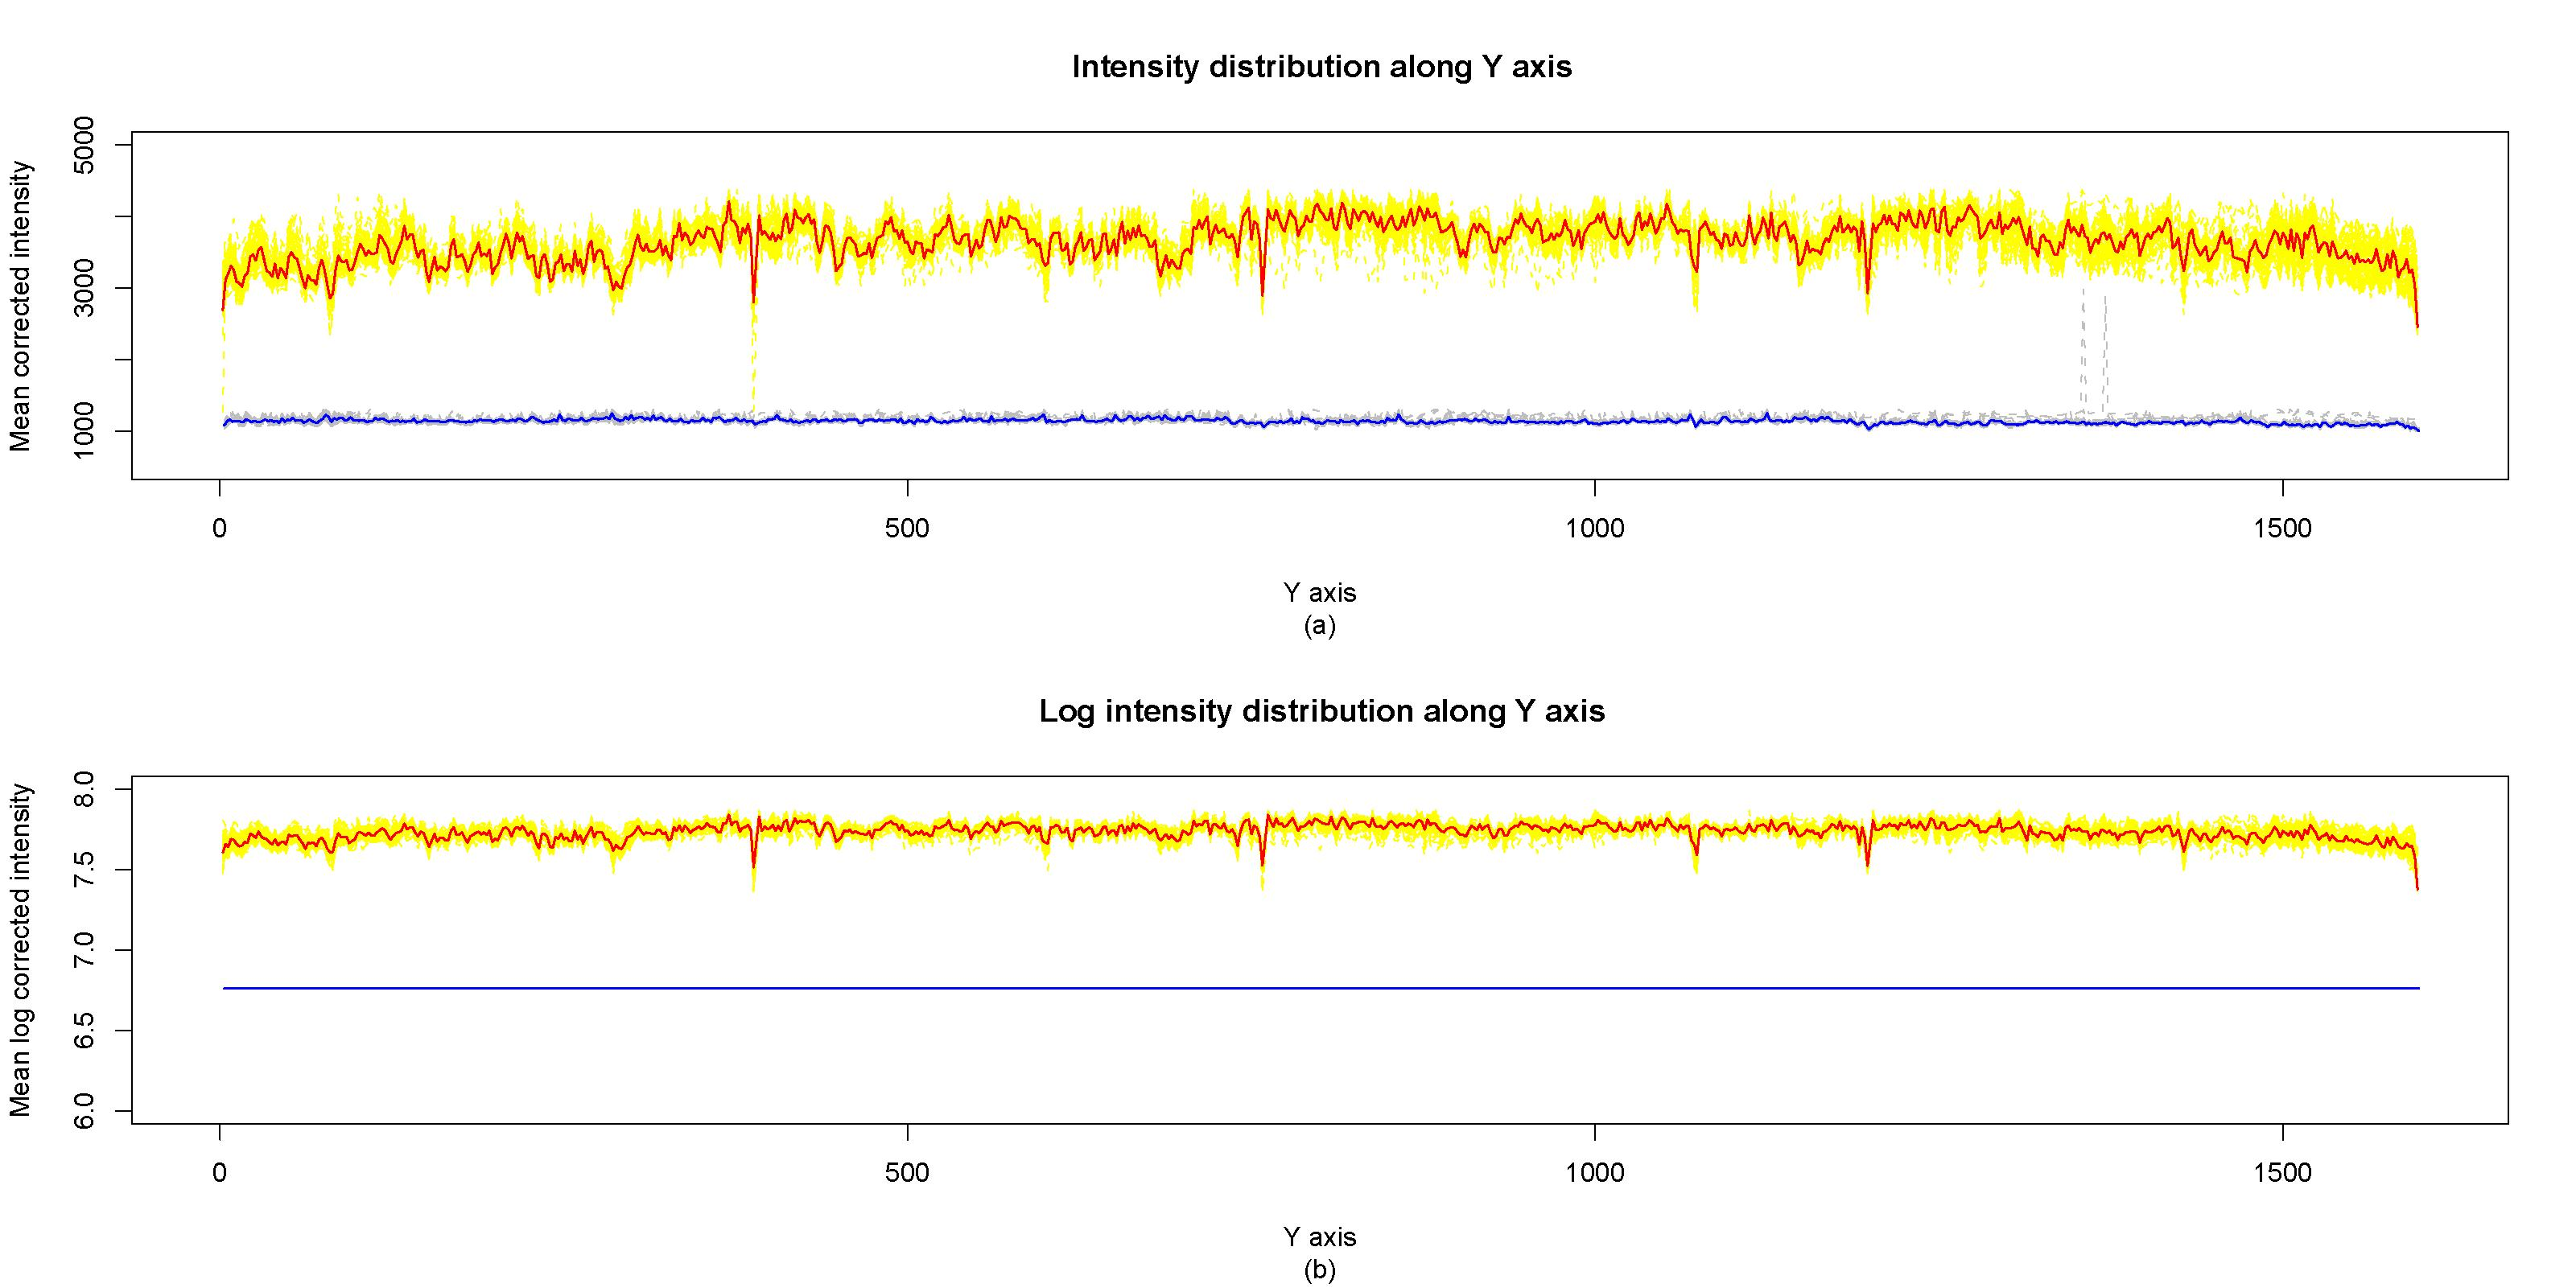
\includegraphics[width=2.5in]{ex.jpg}
%where an .eps filename suffix will be assumed under latex,
%and a .pdf suffix will be assumed for pdflatex; or what has been declared
%via \DeclareGraphicsExtensions.
\caption{Simulation Results.}
\label{fig_sim}
\end{figure}

Note that IEEE typically puts floats only at the top, even when this
results in a large percentage of a column being occupied by floats.


An example of a double column floating figure using two subfigures.
(The subfig.sty package must be loaded for this to work.)
The subfigure \verb+\label+ commands are set within each subfloat command, the
\verb+\label+ for the overall figure must come after \verb+\caption+.
\verb+\hfi+l must be used as a separator to get equal spacing.
The subfigure.sty package works much the same way, except \verb+\subfigure+ is
used instead of \verb+\subfloat+.

%\begin{figure*}[!t]
%\centerline{\subfloat[Case I]\includegraphics[width=2.5in]{NTThang1}%
%\label{fig_first_case}}
%\hfil
%\subfloat[Case II]{\includegraphics[width=2.5in]{NTThang2}%
%\label{fig_second_case}}}
%\caption{Simulation results}
%\label{fig_sim}
%\end{figure*}

Note that often IEEE papers with subfigures do not employ subfigure
captions (using the optional argument to \verb+\subfloat+), but instead will
reference/describe all of them (a), (b), etc., within the main caption.


An example of a floating table. Note that, for IEEE style tables, the
\verb+\caption+ command should come BEFORE the table. Table text will default to
\verb+ \footnotesize+ as IEEE normally uses this smaller font for tables.
 The \verb+\label+ must come after \verb+\caption+ as always.

\begin{table}[!t]
% increase table row spacing, adjust to taste
\renewcommand{\arraystretch}{1.3}
 if using array.sty, it might be a good idea to tweak the value of
 \verb+\extrarowheight+ as needed to properly center the text within the cells
\caption{\uppercase{An Example of a Table}}
\label{table_example}
\centering
 Some packages, such as MDW tools, offer better commands for making tables
 than the plain LaTeX2e tabular which is used here.\\
\vspace{0.8em}
\begin{tabular}{|c||c|}
\hline
One & Two\\
\hline
Three & Four\\
\hline
\end{tabular}
\end{table}


 Note that IEEE does not put floats in the very first column - or typically
 anywhere on the first page for that matter. Also, in-text middle ("here")
 positioning is not used. Most IEEE journals/conferences use top floats
 exclusively. Note that, LaTeX2e, unlike IEEE journals/conferences, places
 footnotes above bottom floats. This can be corrected via the \verb+\fnbelowfloat+
 command of the stfloats package.

\section{Ease of Use}
\subsection{Selecting a Template (Heading 2)}
First, confirm that you have the correct template for your paper size. This template has been tailored for output on the US-letter paper size. If you are using A4-sized paper, please close this template and download the file for A4 paper format called \verb+"CPS_A4_format”+.
\subsection{Maintaining the Integrity of the Specifications}
The template is used to format your paper and style the text. All margins, column widths, line spaces, and text fonts are prescribed; please do not alter them. You may note peculiarities. For example, the head margin in this template measures proportionately more than is customary. This measurement and others are deliberate, using specifications that anticipate your paper as one part of the entire proceedings, and not as an independent document. Please do not revise any of the current designations.

\section{Prepare your paper before styling}
Before you begin to format your paper, first write and save the content as a separate text file. Keep your text and graphic files separate until after the text has been formatted and styled. Do not use hard tabs, and limit use of hard returns to only one return at the end of a paragraph. Do not add any kind of pagination anywhere in the paper. Do not number text heads-the template will do that for you.


Finally, complete content and organizational editing before formatting. Please take note of the following items when proofreading spelling and grammar:
\subsection{Abbreviations and Acronyms}
Define abbreviations and acronyms the first time they are used in the text, even after they have been defined in the abstract. Abbreviations such as IEEE, SI, MKS, CGS, sc, dc, and rms do not have to be defined. Do not use abbreviations in the title or heads unless they are unavoidable.
\subsection{Units}
\begin{itemize}
\item Use either SI (MKS) or CGS as primary units. (SI units are encouraged.) English units may be used as secondary units (in parentheses). An exception would be the use of English units as identifiers in trade, such as “3.5-inch disk drive”.
\item Avoid combining SI and CGS units, such as current in amperes and magnetic field in oersteds. This often leads to confusion because equations do not balance dimensionally. If you must use mixed units, clearly state the units for each quantity that you use in an equation.
\item Do not mix complete spellings and abbreviations of units: “Wb/m2” or “webers per square meter”, not “webers/m2”.  Spell out units when they appear in text: “. . . a few henries”, not “. . . a few H”.
\item Use a zero before decimal points: “0.25”, not “.25”.
\end{itemize}
\subsection{Equations}
The equations are an exception to the prescribed specifications of this template. You will need to determine whether or not your equation should be typed using either the Times New Roman or the Symbol font (please no other font). To create multileveled equations, it may be necessary to treat the equation as a graphic and insert it into the text after your paper is styled.

Number equations consecutively. Equation numbers, within parentheses, are to position flush right, as in (1), using a right tab stop. To make your equations more compact, you may use the solidus ( / ), the exp function, or appropriate exponents. Italicize Roman symbols for quantities and variables, but not Greek symbols. Use a long dash rather than a hyphen for a minus sign. Punctuate equations with commas or periods when they are part of a sentence, as in

Note that the equation is centered using a center tab stop. Be sure that the symbols in your equation have been defined before or immediately following the equation. Use “(1)”, not “Eq. (1)” or “equation (1)”, except at the beginning of a sentence: “Equation (1) is . . .”
\subsection{Some Common Mistakes}
\begin{itemize}
\item The word “data” is plural, not singular.
\item The subscript for the permeability of vacuum 0, and other common scientific constants, is zero with subscript formatting, not a lowercase letter “o”.
\item In American English, commas, semi-/colons, periods, question and exclamation marks are located within quotation marks only when a complete thought or name is cited, such as a title or full quotation. When quotation marks are used, instead of a bold or italic typeface, to highlight a word or phrase, punctuation should appear outside of the quotation marks. A parenthetical phrase or statement at the end of a sentence is punctuated outside of the closing parenthesis (like this). (A parenthetical sentence is punctuated within the parentheses.)
\item A graph within a graph is an “inset”, not an “insert”. The word alternatively is preferred to the word “alternately” (unless you really mean something that alternates).
\item Do not use the word “essentially” to mean “approximately” or “effectively”.
\item In your paper title, if the words “that uses” can accurately replace the word “using”, capitalize the “u”; if not, keep using lower-cased.
\item Be aware of the different meanings of the homophones “affect” and “effect”, “complement” and “compliment”, “discreet” and “discrete”, “principal” and “principle”.
\item Do not confuse “imply” and “infer”.
\item The prefix “non” is not a word; it should be joined to the word it modifies, usually without a hyphen.
\item There is no period after the “et” in the Latin abbreviation “et al.”.
\item The abbreviation “i.e.” means “that is”, and the abbreviation “e.g.” means “for example”.
\end{itemize}

\section{Kết luận}
The conclusion goes here. this is more of the conclusion

% conference papers do not normally have an appendix


% use section* for acknowledgement
\section*{Cảm tạ}


The authors would like to thank...
more thanks here


% trigger a \newpage just before the given reference
% number - used to balance the columns on the last page
% adjust value as needed - may need to be readjusted if
% the document is modified later
%\IEEEtriggeratref{8}
% The "triggered" command can be changed if desired:
%\IEEEtriggercmd{\enlargethispage{-5in}}

% references section

% can use a bibliography generated by BibTeX as a .bbl file
% BibTeX documentation can be easily obtained at:
% http://www.ctan.org/tex-archive/biblio/bibtex/contrib/doc/
% The IEEEtran BibTeX style support page is at:
% http://www.michaelshell.org/tex/ieeetran/bibtex/
%\bibliographystyle{IEEEtran}
% argument is your BibTeX string definitions and bibliography database(s)
%\bibliography{IEEEabrv,../bib/paper}
%
% <OR> manually copy in the resultant .bbl file
% set second argument of \begin to the number of references
% (used to reserve space for the reference number labels box)

\balance

\begin{thebibliography}{1}

\bibitem{IEEEhowto:kopka}
H.~Kopka and P.~W. Daly, \emph{A Guide to \LaTeX}, 3rd~ed.\hskip 1em plus
  0.5em minus 0.4em\relax Harlow, England: Addison-Wesley, 1999.

\end{thebibliography}




% that's all folks
\end{document}